% Preamble
\documentclass[11pt]{article}

% Packages
\usepackage[UTF8]{ctex}
\usepackage{amsmath}
\usepackage{amsfonts}
\usepackage{amssymb}
\usepackage{amsthm}
\usepackage{tikz}
\usepackage{subcaption}
\usepackage{float}

\newtheorem{definition}{定义}
\newtheorem{property}{性质}
\newtheorem{lemma}{引理}
\newtheorem{theorem}{定理}

\numberwithin{equation}{section}
\numberwithin{theorem}{section}

\title{各类曲线的性质}
\author{Renatus Madrigal}
\date{\today}

% Document
\begin{document}

\maketitle
\tableofcontents

\section{基础公式}\label{sec:basic-formula}

在这一节,我们将介绍一些基本的公式。仅供参考,不需要严格证明。

\begin{theorem}\label{thm:area-formula}
  对于一条曲线 $L$ ,参数方程为 $(x(t), y(t))$ ,极坐标方程有 $\rho = f(\theta)$ ,有:

  \begin{equation}
    \begin{aligned}
      S &= \int_L y \ \mathrm{d} x \\
      &= \int_L y \frac{\mathrm{d}x}{\mathrm{d}t}\ \mathrm{d}t \\
      &= \frac{1}{2}\int_L r^2\ \mathrm{d}\theta
    \end{aligned}
  \end{equation}

\end{theorem}

\begin{theorem}\label{thm:length-formula}
  对于曲线 $L$ , 有弧长的微分:

  \begin{equation}
    \begin{aligned}
      \mathrm{d} l &= \sqrt{1 + \left( \frac{\mathrm{d}y}{\mathrm{d}x}\right)^2} \mathrm{d}x \\
      &= \sqrt{\left(\frac{\mathrm{d}x}{\mathrm{d}t}\right)^2
      + \left(\frac{\mathrm{d}y}{\mathrm{d}t}\right)^2} \mathrm{d}t \\
      &= \sqrt{r^2 + \left(\frac{\mathrm{d}r}{\mathrm{d}\theta}\right)^2} \mathrm{d}\theta
    \end{aligned}
  \end{equation}

  且有对于弧长 $l$ 有:

  \begin{equation}
    l = \int_L \mathrm{d}l
  \end{equation}
\end{theorem}

\section{星形线}\label{sec:star-curve}

\begin{definition}
  \label{def:star-curve}
  星形线是内摆线的一种特例,是一个小圆在一个大圆上滚动时,所描出的点的轨迹,其中小圆和大圆的半径满足: $r = \frac{R}{4}$。
\end{definition}

星形线的图像如下:

\begin{figure}[ht]
  \label{fig:star-curve-all}
  \centering
  \begin{subfigure}[t]{0.45\textwidth}
    \label{fig:star-curve}
    \centering
    \begin{tikzpicture}[scale=1]
      \draw[->] (-2,0) -- (2,0) node[right] {$x$};
      \draw[->] (0,-2) -- (0,2) node[above] {$y$};
      \draw[blue, thick, domain=0:2*pi, samples=200]
      plot ( {cos(\x r)^3}, {sin(\x r)^3} );
    \end{tikzpicture}
    \caption{星形线的图像}
  \end{subfigure}
  \hfill
  \begin{subfigure}[t]{0.45\textwidth}
    \label{fig:star-curve-construction}
    \centering
    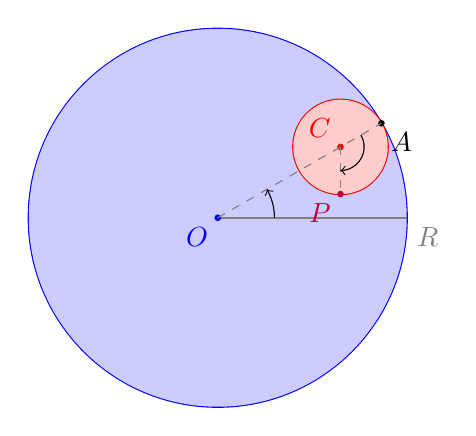
\begin{tikzpicture}[scale=1.2]
      % 定义大圆和小圆半径
      \def\R{2}     % 大圆半径
      \def\r{0.5}   % 小圆半径
      \def\theta{30} % 大圆旋转角度(度)

      % 计算小圆圆心坐标
      \pgfmathsetmacro{\cx}{(\R - \r)*cos(\theta)}
      \pgfmathsetmacro{\cy}{(\R - \r)*sin(\theta)}

      % 计算小圆自转角度
      \pgfmathsetmacro{\phi}{\R/\r * \theta}

      % 轨迹点P的坐标
      \pgfmathsetmacro{\px}{\cx + \r*cos(-\phi + \theta)}
      \pgfmathsetmacro{\py}{\cy + \r*sin(-\phi + \theta)}

      % 绘制大圆
      \draw[thick, blue] (0,0) circle (\R);
      \fill[blue!20] (0,0) circle (\R); % 填充大圆
      \draw[thick, gray] (0,0) -- (\R, 0) node[below right] {$R$};

      % 绘制小圆
      \draw[red, thick] (\cx, \cy) circle (\r);
      \fill[red!20] (\cx, \cy) circle (\r);

      % 标记大圆和小圆圆心
      \fill[blue] (0,0) circle (1pt) node[below left] {$O$};
      \fill[red] (\cx, \cy) circle (1pt) node[above left] {$C$};

      % 绘制接触点(大圆与小圆的切点)
      \pgfmathsetmacro{\contactX}{\R*cos(\theta)}
      \pgfmathsetmacro{\contactY}{\R*sin(\theta)}
      \fill[black] (\contactX, \contactY) circle (1pt) node[below right] {$A$};

      % 绘制轨迹点P
      \fill[purple] (\px, \py) circle (1pt) node[below left] {$P$};

      % 绘制辅助线:大圆圆心到接触点
      \draw[dashed, gray] (0,0) -- (\contactX, \contactY);

      % 绘制辅助线:小圆圆心到轨迹点P
      \draw[dashed, gray] (\cx, \cy) -- (\px, \py);

      % 绘制角度标记(大圆旋转角度θ)
      \draw[->, black] (0:0.3*\R) arc (0:\theta:0.3*\R);

      % 绘制角度标记(小圆自转角度φ)
      \draw[->, black] (\cx/2 + \contactX/2, \cy/2 + \contactY/2) arc (\theta:\theta-\phi:0.5*\r);
    \end{tikzpicture}
    \caption{星形线的几何构造}
  \end{subfigure}
  \caption{星形线的图像和几何构造}
\end{figure}

\begin{property}\label{prop:star-curve-parametric-equation}
  星形线的参数方程为:
  \begin{equation}\label{eq:star-curve-parametric-equation}
    \begin{cases}
      x = R\cos^3(t) \\
      y = R\sin^3(t)
    \end{cases}
  \end{equation}
\end{property}

\begin{proof}
  设小圆的半径为 $r$,大圆的半径为 $R$,小圆在大圆上滚动时,所描出的点的轨迹为 $(x(t), y(t))$。
  设小圆滚动角度为 $\theta$,小圆自转角度为 $\phi$,由无滑动滚动的性质,有:

  \begin{equation}\label{eq:rolling-condition}
    \phi = \frac{R}{r} \theta
  \end{equation}

  又有定义:$r = \frac{R}{4}$ ,所以 $\phi = 4\theta$ 。

  此时,又有坐标关系:

  \begin{equation}\label{eq:star-curve-rolling-condition}
    \begin{cases}
      x = x_c + r \cos(\theta - \phi) \\
      y = y_c + r \sin(\theta - \phi)
    \end{cases}
  \end{equation}

  将 $\phi = 4\theta$ 代入 \eqref{eq:star-curve-rolling-condition},得到:

  \begin{equation}\label{eq:star-curve-rolling-condition-2}
    \begin{cases}
      x = x_c + r \cos(-3\theta) \\
      y = y_c + r \sin(-3\theta)
    \end{cases}
  \end{equation}

  又有 $C$ 点坐标为 $(x_c, y_c) = (3r \cos(\theta), 3r \sin(\theta))$,代入 \eqref{eq:star-curve-rolling-condition-2},得到:

  \begin{equation}\label{eq:star-curve-rolling-condition-3}
    \begin{cases}
      x = 3r \cos(\theta) + r \cos(-3\theta) \\
      y = 3r \sin(\theta) + r \sin(-3\theta)
    \end{cases}
  \end{equation}

  应用三倍角公式展开,得到:

  \begin{equation}\label{eq:star-curve-rolling-condition-4}
    \begin{cases}
      x = 3r \cos(\theta) + r (4\cos^3(\theta) - 3\cos(\theta)) \\
      y = 3r \sin(\theta) + r (4\sin^3(\theta) - 3\sin(\theta))
    \end{cases}
  \end{equation}

  即得式 \eqref{eq:star-curve-parametric-equation}。

\end{proof}

由参数方程 \eqref{eq:star-curve-parametric-equation} 容易得到:

\begin{property}\label{prop:star-curve-coordinate-equation}
  星形线的坐标方程为:
  \begin{equation}\label{eq:star-curve-coordinate-equation}
    x ^ {\frac{2}{3}} + y ^ {\frac{2}{3}} = R
  \end{equation}
\end{property}

由定理 \ref{thm:area-formula} 、 \ref{thm:length-formula} 有:

\begin{property}\label{prop:star-curve-area}
  星形线的面积为:
  \begin{equation}\label{eq:star-curve-area}
    \begin{aligned}
      S &= 4R^2 \int_{0}^{\frac{\pi}{2}} y \frac{dx}{dt} dt \\
      &= 4R^2 \int_{0}^{\frac{\pi}{2}} \sin^3t \cdot 3\cos^2t dt \\
      &= 12R^2 \cdot \int_{0}^{\frac{\pi}{2}} (sin^4t - sin^6t) dt \\
      &= 12R^2 \cdot \left( \frac{3}{16}\pi - \frac{15}{96}\pi \right) \\
      &= \frac{3}{8} \pi R^2
    \end{aligned}
  \end{equation}
\end{property}

和

\begin{property}\label{prop:star-curve-length}
  星形线的长度为:
  \begin{equation}\label{eq:star-curve-length}
    \begin{aligned}
      l &= 3R \int_0^{2\pi} \sqrt{(\cos^2t\sin t)^2 + (\sin^2t\cos t)^2} \mathrm{d}t \\
      &= \frac{3}{2}R\int_0^{2\pi}\left|\sin 2t\right| \mathrm{d}t \\
      &= 6R
    \end{aligned}
  \end{equation}
\end{property}

\section{三叶玫瑰线}\label{sec:three-leaved-rose}

\begin{definition}\label{def:three-leaved-rose}
  三叶玫瑰线满足极坐标方程:
  \begin{equation}\label{def:three-leaved-rose-polar-equation}
    r = R\cos(3\theta)
  \end{equation}
\end{definition}

三叶玫瑰线没有简单的纯几何手段定义。它的图像如下:

\begin{figure}[H]
  \centering
  \begin{tikzpicture}[scale=1.5]

    \def\R{1.5} % 设置参数 R
    \draw[->] (-2,0) -- (2,0) node[right] {$x$};
    \draw[->] (0,-2) -- (0,2) node[above] {$y$};
    \draw[domain=0:360, samples=200, smooth, variable=\t, blue, thick]
    plot ({\R*cos(3*\t)*cos(\t)}, {\R*cos(3*\t)*sin(\t)});

  \end{tikzpicture}
  \caption{三叶玫瑰线的图像}
\end{figure}

\section{双纽线}\label{sec:double-curve}




\end{document}
